\subsubsection{Плотнейшая упаковка}

Термин плотнейшая упаковка характеризует специфическое расположение элементов в пространстве или на поверхности таким образом, чтобы отношение заполненной области к незаполненной было максимальным. 

При рассмотрении упаковок дисков на поверхности легко определить, что расположение сфер в центрах квадратной решётки с диаметром равным стороне данной решётки не является плотнейшим методом расположения данных элементов.

Плотнейшие упаковки в кристаллографии -- формы расположения атомов в кристаллической решётке, которые характеризуются наибольшим числом атомов в единице объёма кристалла. Такие упаковки отчётливо выражены в большом числе кристаллических структур. Они характерны для большинства металлов, а также для кристаллизованных инертных газов. Структуры многих неорганических (ионных) кристаллов представляют собой плотнейшие упаковки шаровых анионов (с большими ионными радиусами), в пустотах которых распределяются мелкие катионы.

Более 300 лет известна (И. Кеплер) и признаётся наиболее плотной упаковка шаров «вручную», когда на слой шаров, уложенных по углам квадратной сетки, наложен другой такой же слой шаров в лунки нижележащего (коэффициент заполнения пространства таким образом $74,05\%$).

\begin{figure}[h]
    \begin{subfigure}{0.49\textwidth}
        \begin{center}
            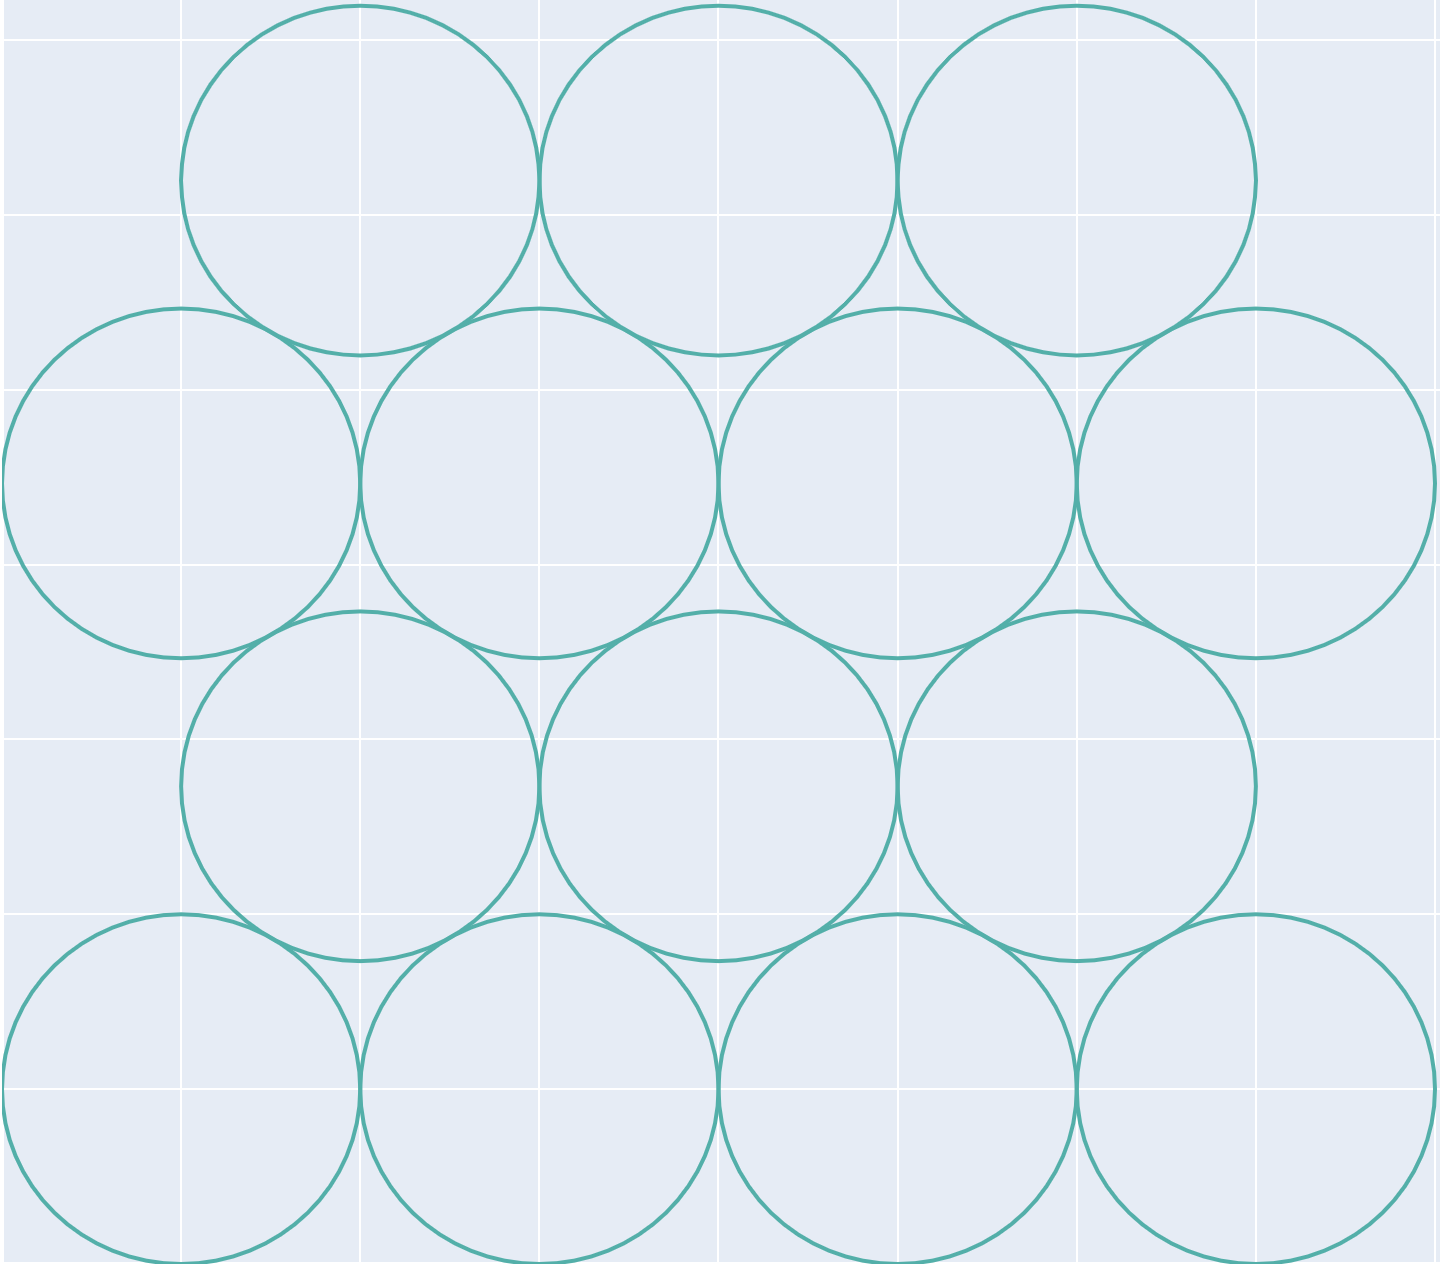
\includegraphics
            [width=8cm,height=8cm]
            {figures/circles_tighest_packing.png} 
        \end{center}
        \caption{\label{fig:tighest_circles}
        Плотнейшая упаковка окружностей}
    \end{subfigure}
    \begin{subfigure}{0.49\textwidth}
        \begin{center}
            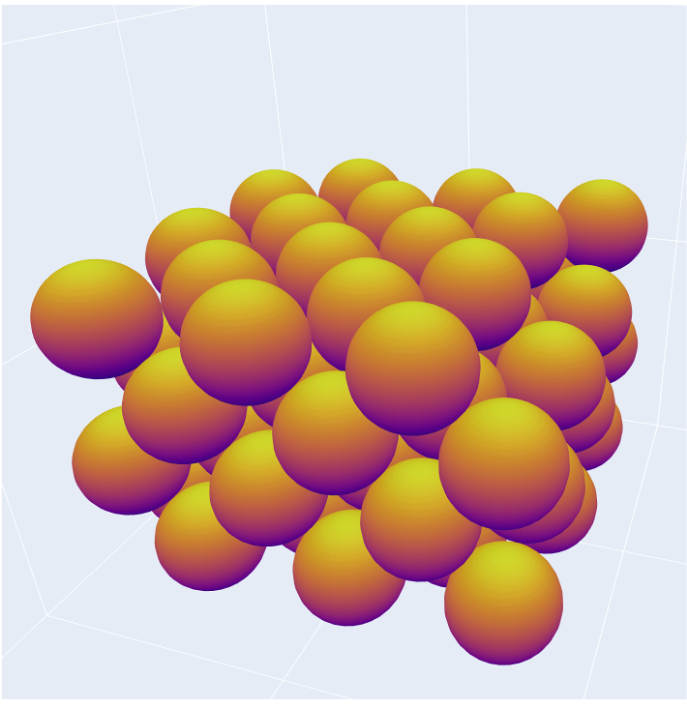
\includegraphics
            [width=8cm,height=8cm] 
            {figures/spheres_tighest_packing.png}
        \end{center}
        \caption{\label{fig:tighest_spheres}
        Плотнейшая упаковка сфер}
    \end{subfigure}
\caption{
\label{fig:main_figure}
Пример плотнейшей упаковки.
}
\end{figure}

Очевидно, что шары третьего слоя будут лежать точно над шарами первого. Такая упаковка обычно называется кубической плотнейшей гранецентрированной. Она считалась единственной, пока в 1900 английский кристаллограф У. Барлоу не показал, что, поставив куб на угол, его можно разобрать на плоские ещё более плотные слои, в которых лунок между шарами в два раза больше числа самих шаров. Варьируя укладку плотноупакованных слоев, получают бесчисленное множество плотнейших упаковок с одинаковым коэффициентом заполнения – $74,05\%$. Если ограничить наслаивание некоторым периодом, то получается: двухслойная плотнейшая упаковка, трёхслойная, четырёхслойная и так далее. Трёхслойная упаковка – это исходная кубическая, прочие – все гексагональные.

